%! Author = antonio
%! Date = 7/1/24

In our analysis process, one first begins to represent what are the data related to the various features
and how among the various features the data are distributed by making a visual representation in pairs of features.

\begin{enumerate}
%    FEATURE 1 AND 2
    \item Starting with the analysis of the first two features and creating a histogram and a scatter
    \autoref{fig:feature1vs2}, one can see:
    \begin{itemize}
        \item Both features overlap
        \item Follow a Gaussian distribution
        \item Feature 1 has a peak at [-0.213, 0.276] and it is worth 0.541 for the false class, instead for Feature 2
        the peak at [-0.402, 0.165] and it is worth 0.516 for the true class.
    \end{itemize}
    Seeing \autoref{fig:feature1vs2} again, it would appear that \autoref{fig:feature1vs2a} and
    \autoref{fig:feature1vs2b} appear to be visually the same but in b they are represented centred
    which as can be seen is quite similar because Feature 1 has \(\mu = 0.00170711\)
    and \(\sigma^2 = 1.00134304\), instead Feature 2 has \(\mu = 0.00503903\) and \(\sigma^2 =  0.9983527\)
    \begin{figure}[h!]
        \centering
        \begin{subfigure}[b]{0.4\linewidth}
            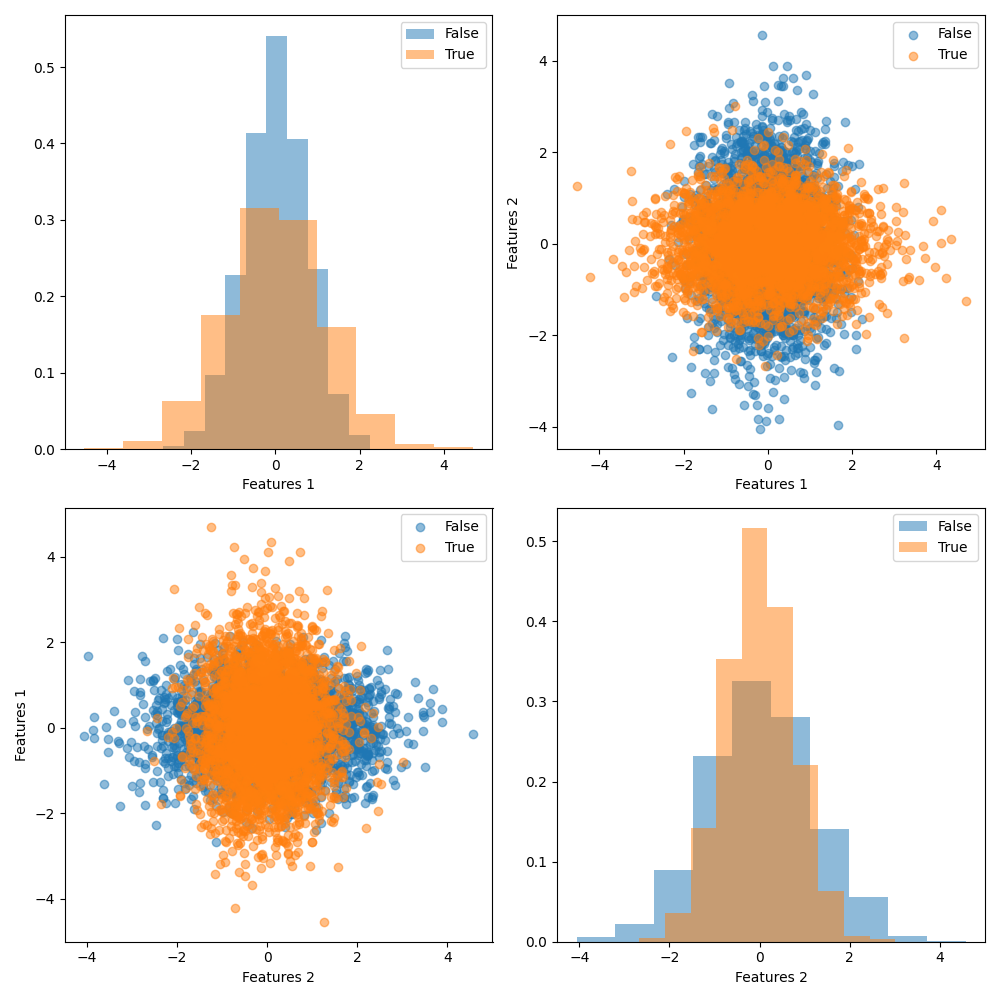
\includegraphics[width=\linewidth]{Lab/02. Lab 02/Images/01. Graphics Features 1_2 Without Mean}
            \caption{Without mean}
            \label{fig:feature1vs2a}
        \end{subfigure}
        \begin{subfigure}[b]{0.4\linewidth}
            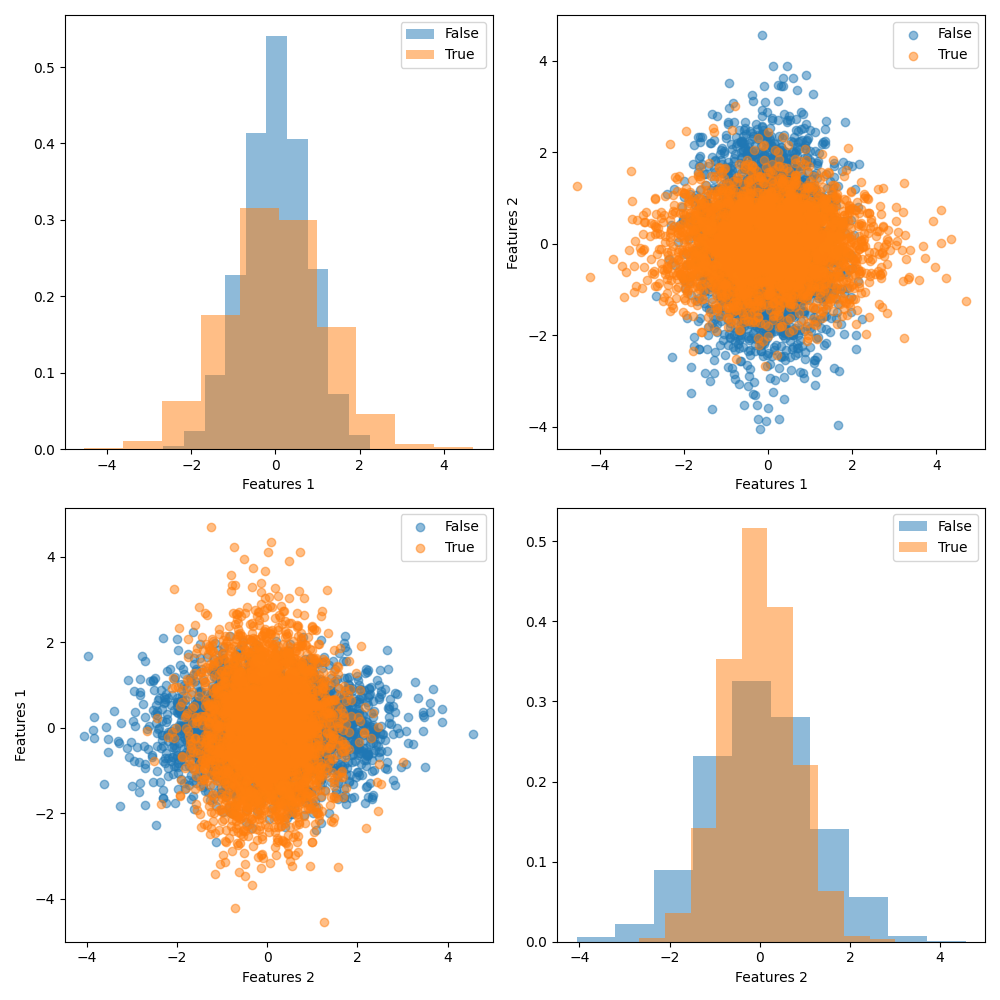
\includegraphics[width=\linewidth]{Lab/02. Lab 02/Images/02. Graphics Features 1_2 With Mean}
            \caption{With mean}
            \label{fig:feature1vs2b}
        \end{subfigure}
        \caption{Feature 1 vs Feature 2 - Without centering the data relative to the average (a)
            and with centering the data relative to the average (b)}
        \label{fig:feature1vs2}
    \end{figure}


%    FEATURE 3 AND 4
    \item For features 3 and 4, observed in \autoref{fig:feature3vs4}, on the other hand, they have:
    \begin{itemize}
        \item do not overlap like the previous two
        \item Follow a Gaussian distribution but the true and false labels are centred at different
        points
        \item Feature 3 has a peak at [-1.063, -0.568] and it is worth 0.517 for the false class,
        instead for Feature 4 the peak at [0.290, 0.783] and it is worth 0.525 for the false class.
    \end{itemize}
    Seeing \autoref{fig:feature3vs4a} and \autoref{fig:feature3vs4b}, data are already similar because, the mean
    calculated with reference to the two classes is close to 0, in fact:
    Feature 3 has \(\mu = -0.00560753\) and \(\sigma^2 = 1.0024818\), instead
    Feature 4 has \(\mu = 0.00109537\) and \(\sigma^2 = 0.99029389\)
    \begin{figure}[h!]
        \centering
        \begin{subfigure}[b]{0.4\linewidth}
            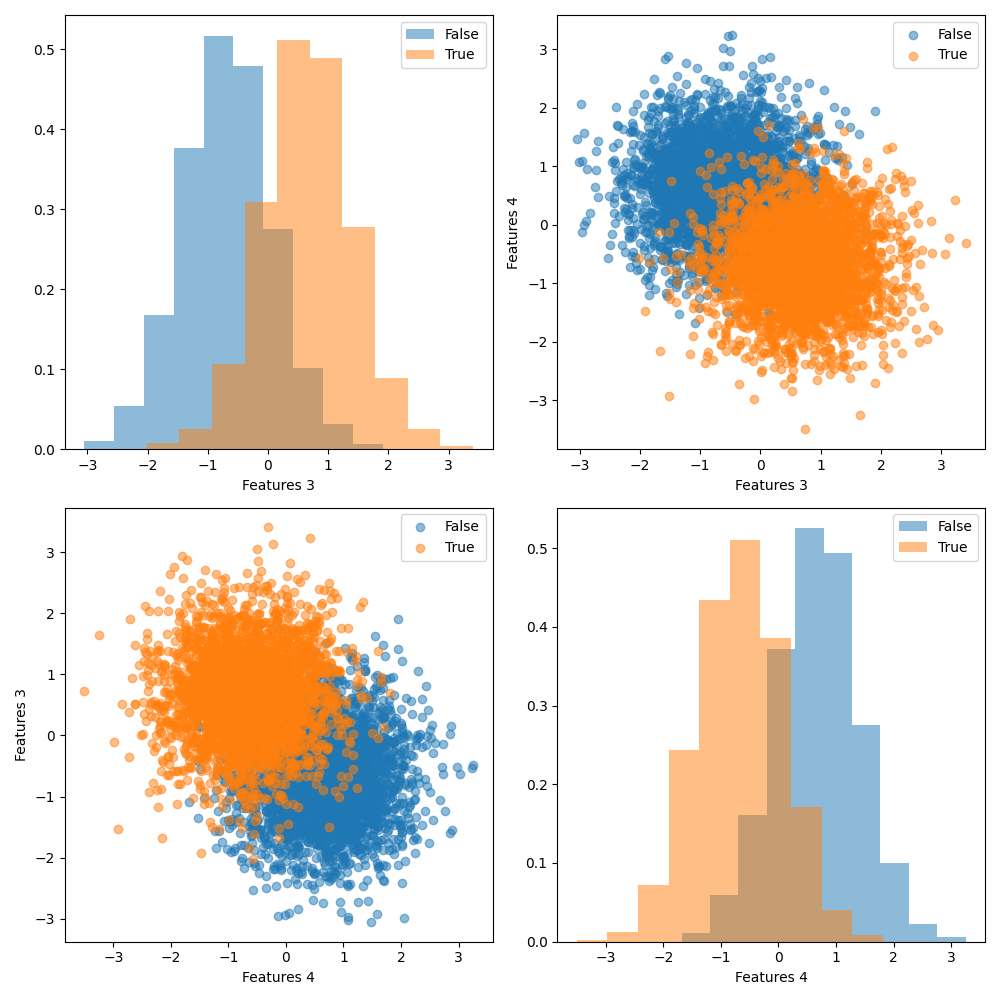
\includegraphics[width=\linewidth]{Lab/02. Lab 02/Images/03. Graphics Features 3_4 Without Mean}
            \caption{Without mean}
            \label{fig:feature3vs4a}
        \end{subfigure}
        \begin{subfigure}[b]{0.4\linewidth}
            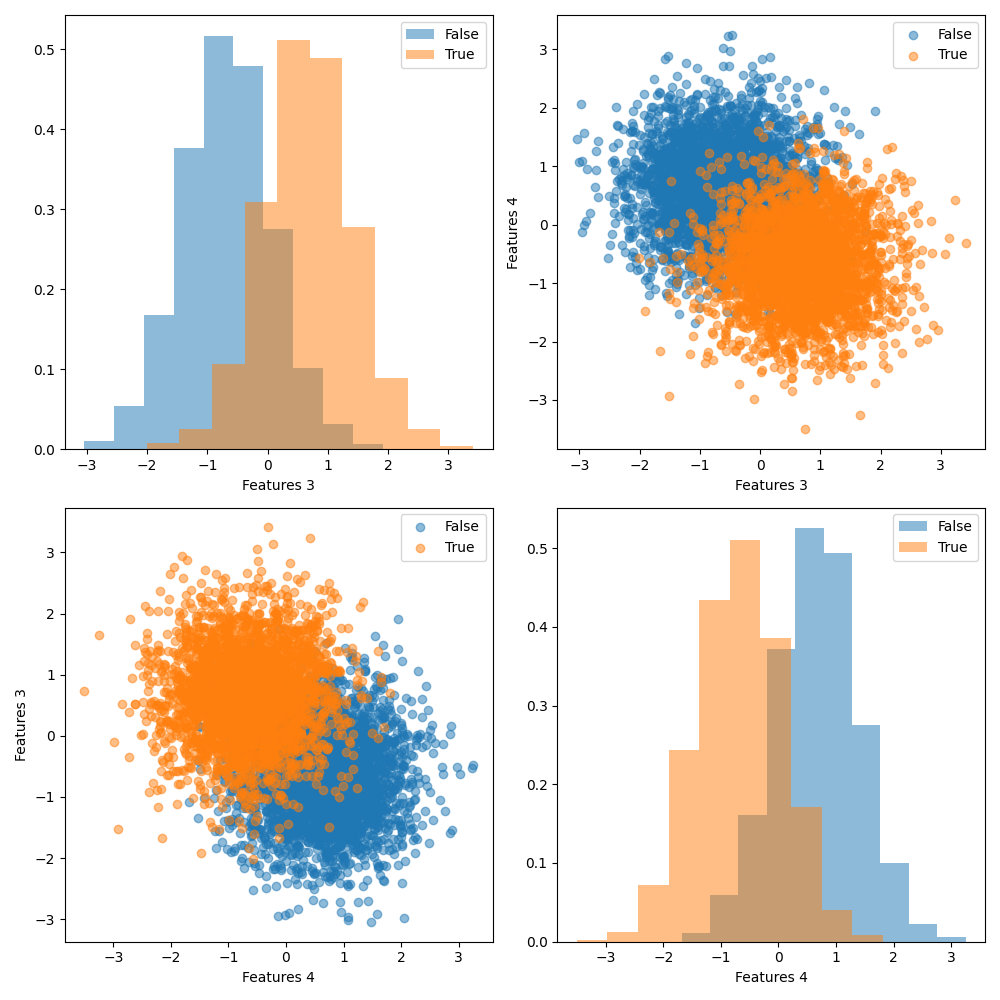
\includegraphics[width=\linewidth]{Lab/02. Lab 02/Images/04. Graphics Features 3_4 With Mean}
            \caption{With mean}
            \label{fig:feature3vs4b}
        \end{subfigure}
        \caption{Feature 3 vs Feature 4 - Without centering the data relative to the average (a)
            and with centering the data relative to the average (b)}
        \label{fig:feature3vs4}
    \end{figure}


%    FEATURE 5 AND 6
    \item  For features 5 and 6, observed in \autoref{fig:feature5vs6}, one can see:
    \begin{itemize}
        \item Do not totally overlap
        \item For both features, the true labels don't follow a Gaussian distribution as opposed to the false ones,
        which could be more approximate
        \item Feature 5 has a peak at [-1.211, -0.783] and it is worth 0.572 for the true class, instead
        for Feature 6 has a peak at [-1.273, -0.817] and it is worth 0.553 for the true class.
    \end{itemize}
    Also in this other case, \autoref{fig:feature5vs6a} and \autoref{fig:feature5vs6b} are similar because again the
    average is close to 0.
    Feature 5 has \(\mu = -0.00700025\) and Feature 6 has \(\mu = 0.00910515\)

    \begin{figure}[t]
        \centering
        \begin{subfigure}[b]{0.4\linewidth}
            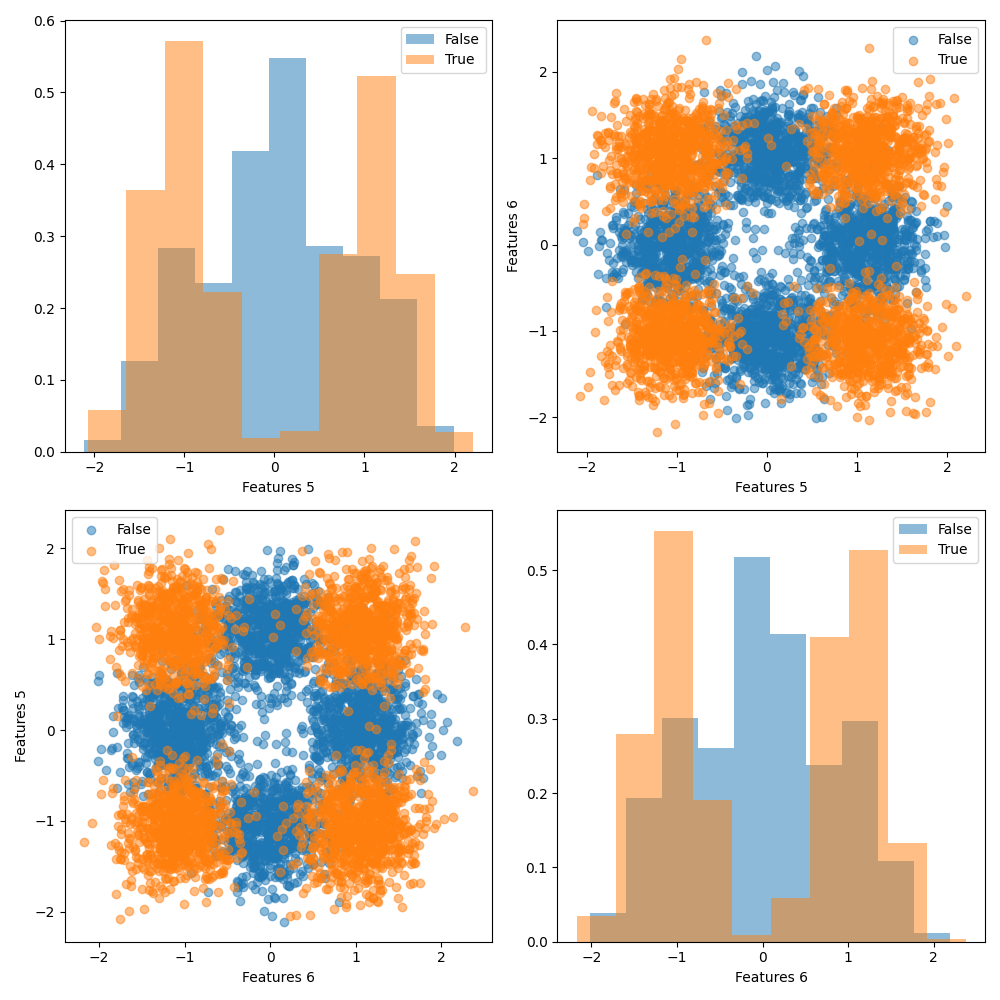
\includegraphics[width=\linewidth]{Lab/02. Lab 02/Images/05. Graphics Features 5_6 Without Mean}
            \caption{Without mean}
            \label{fig:feature5vs6a}
        \end{subfigure}
        \begin{subfigure}[b]{0.4\linewidth}
            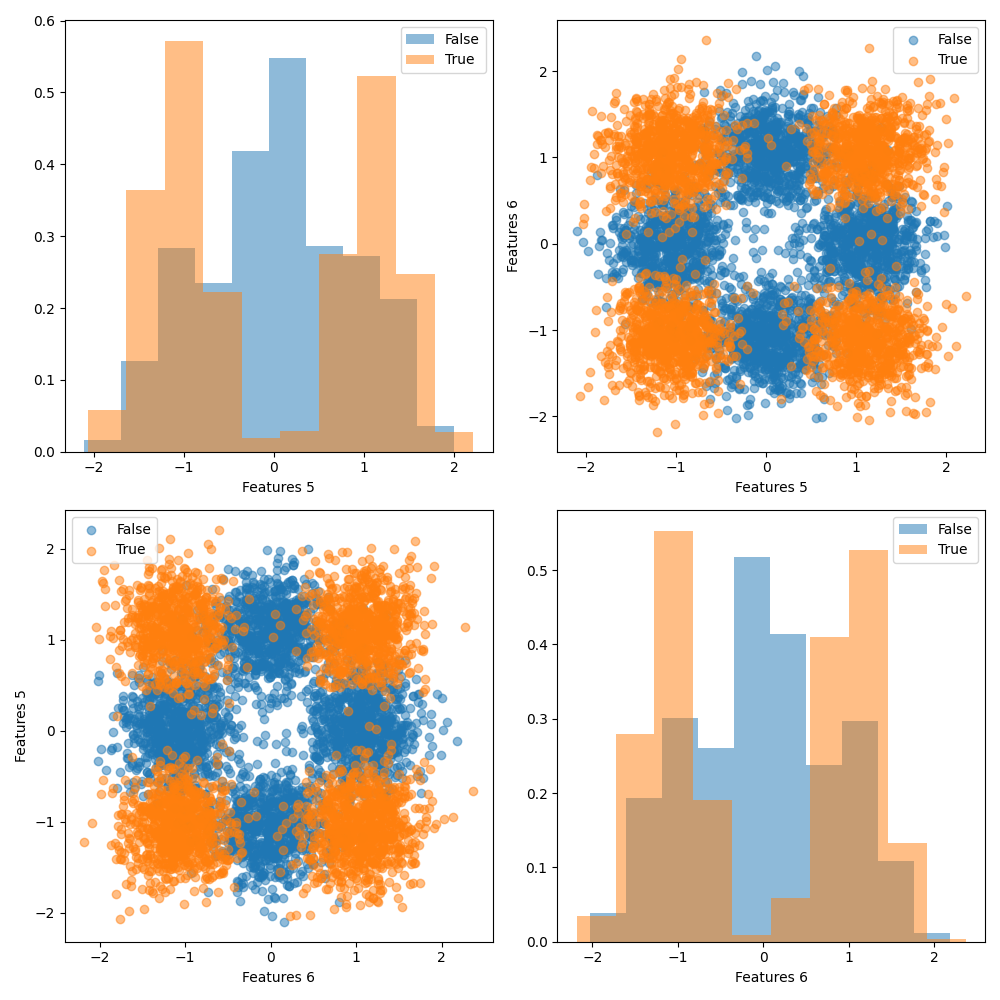
\includegraphics[width=\linewidth]{Lab/02. Lab 02/Images/06. Graphics Features 5_6 With Mean}
            \caption{With mean}
            \label{fig:feature5vs6b}
        \end{subfigure}
        \caption{Feature 5 vs Feature 6 - Without centering the data relative to the average (a)
            and with centering the data relative to the average (b)}
        \label{fig:feature5vs6}
    \end{figure}

\end{enumerate}